\chapter{how to make tempest in 1981}
\label{sec:building}
\lstset{style=6502Style}
\lhead[tempest]{}

It is 1981 and Atari Corporation has tasked you with writing a state-of-the-art video game.
To complete your assignment they have equipped you with a pencil and a bundle of sheets. You
wonder where the computer is, and at what point they will give you one. 

You can sit in your office and wonder in vain, because they are never going to give you one.
You must devise and program the game entirely with pencil and paper. There is only one computer
in the building, and it is the price of a house. They are not going to let
you anywhere near that computer. You are in building 1272 and the computer is in building 1360.
You are not even on the same block as the computer.
\begin{figure}[H]
      \centering
      \frame{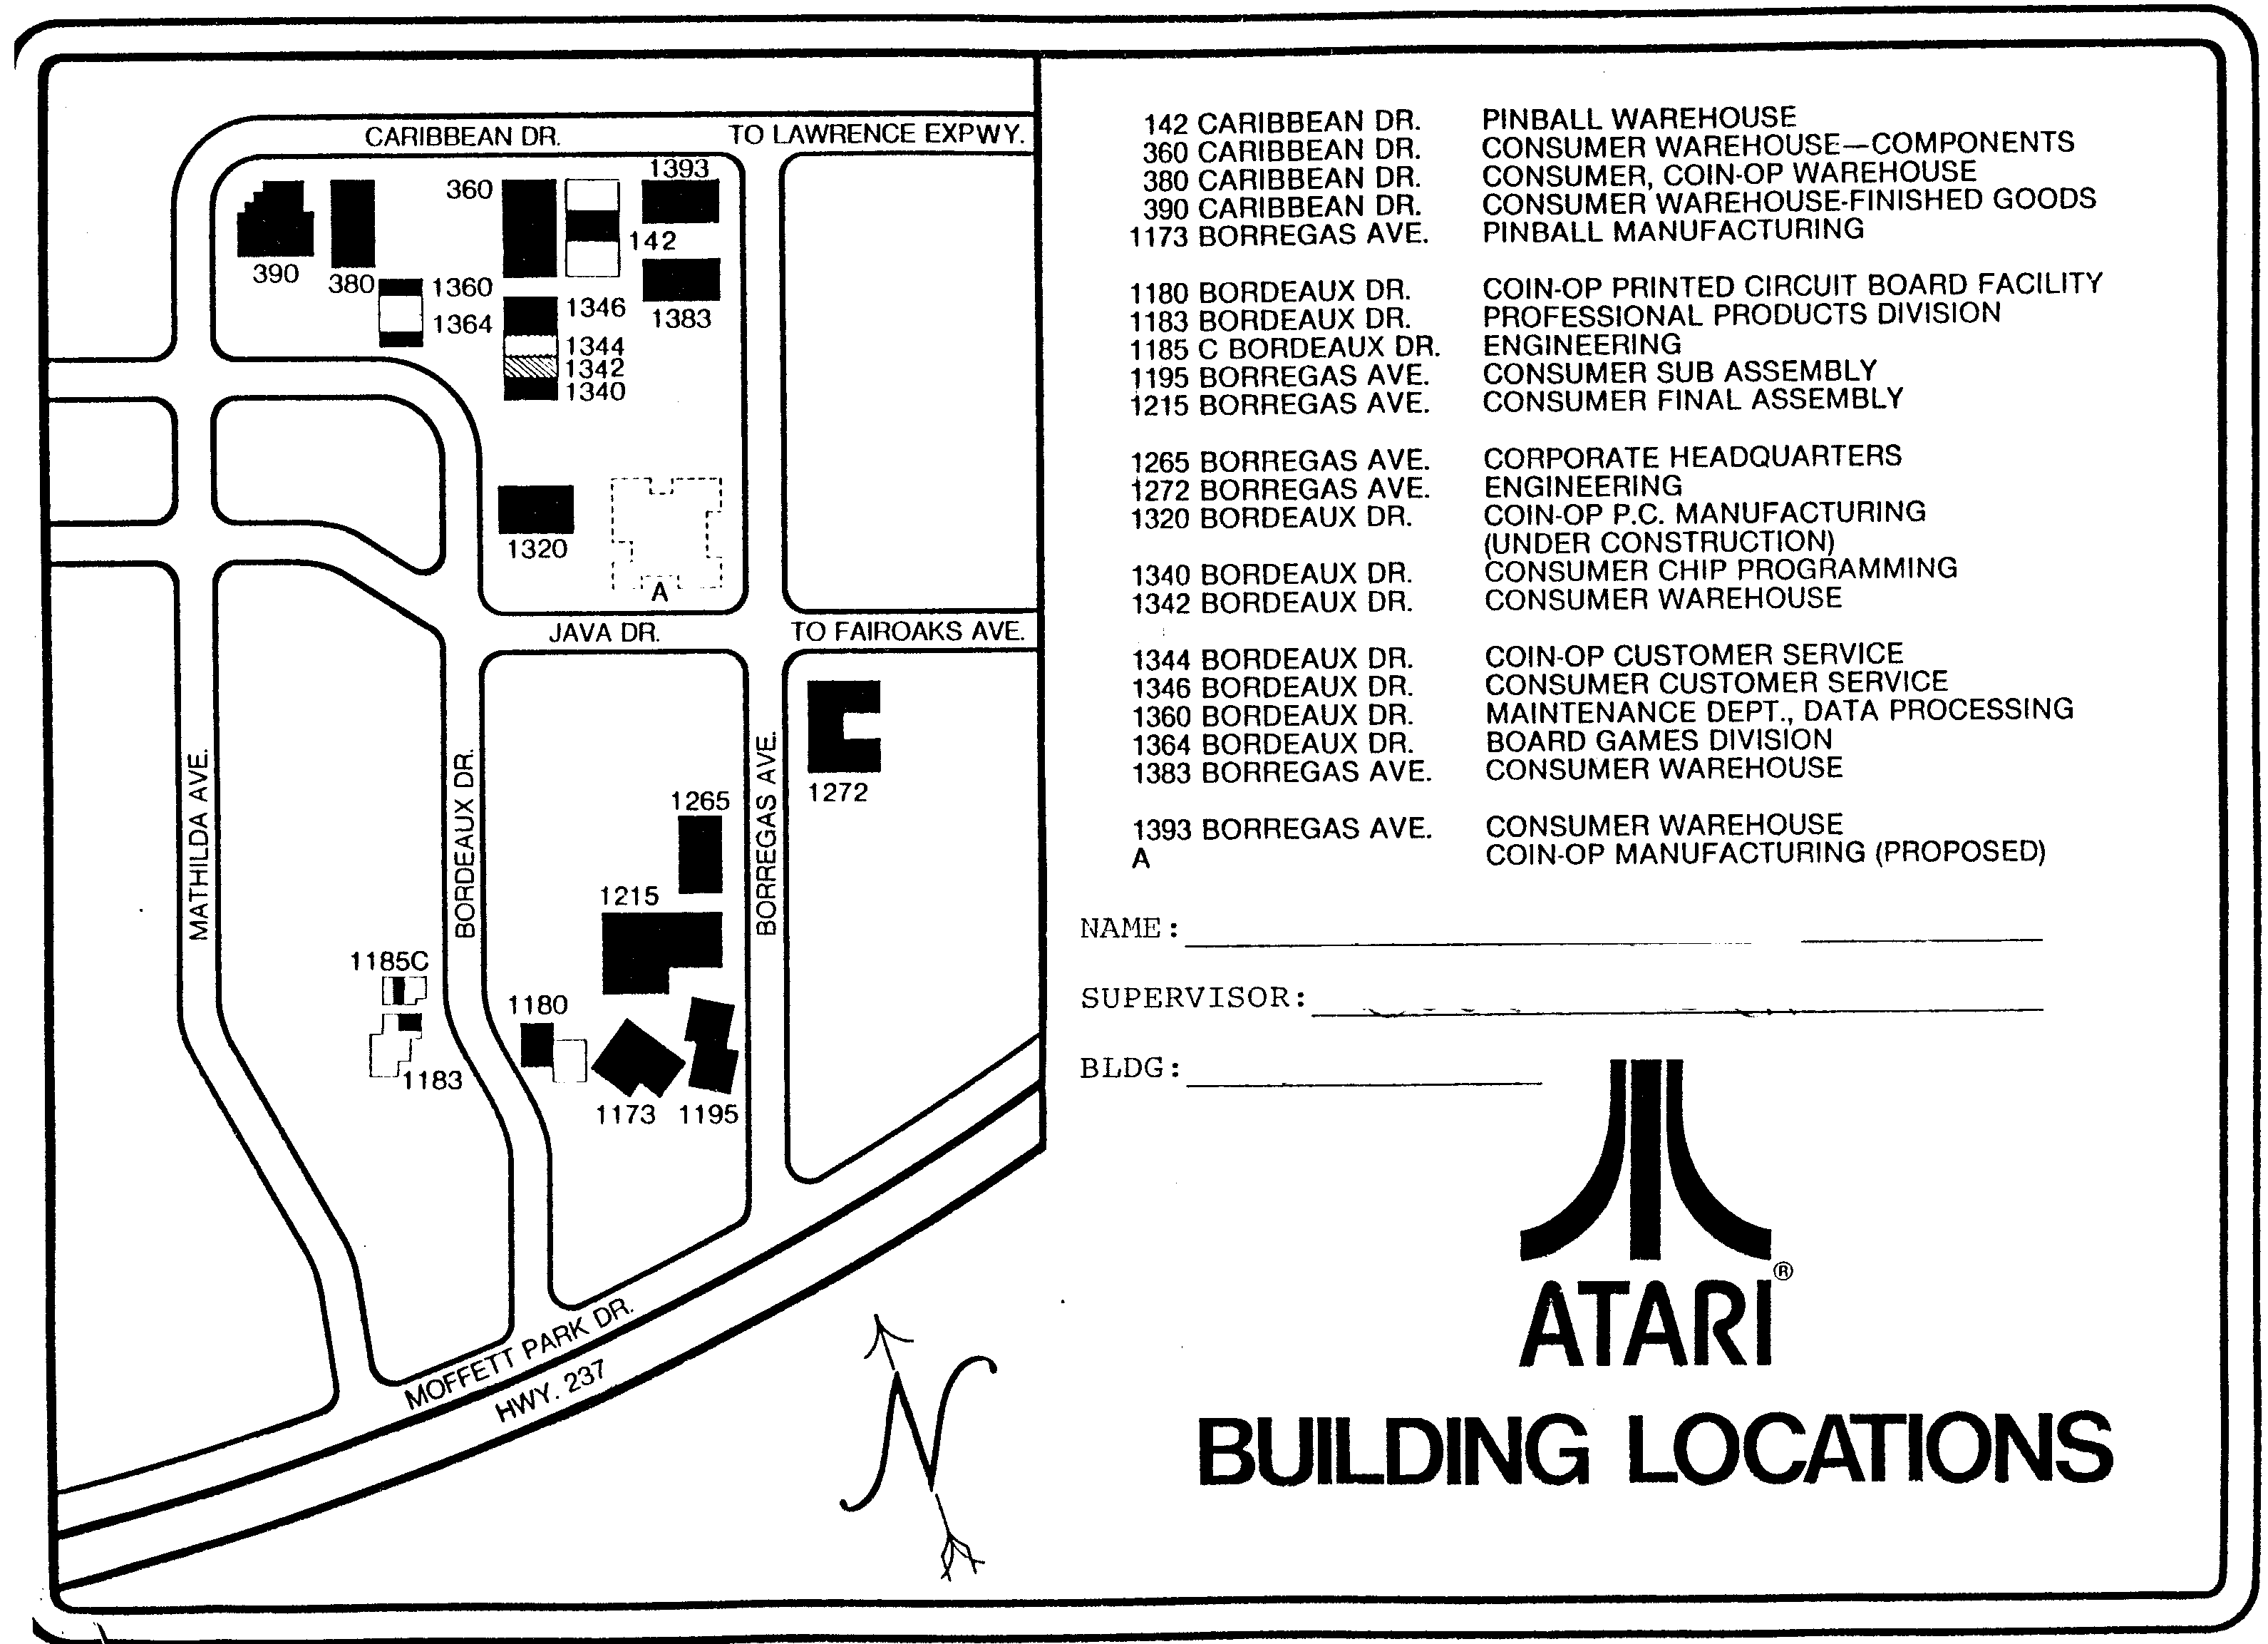
\includegraphics[width=8cm]{src/build/map.png}}%
    \caption{The computer is in another building.}
\end{figure}

Instead you are confronted with a ream of blank sheets such as this one; into which you must pencil
the assembly language instructions that will make your game happen.
\begin{figure}[H]
      \centering
      \frame{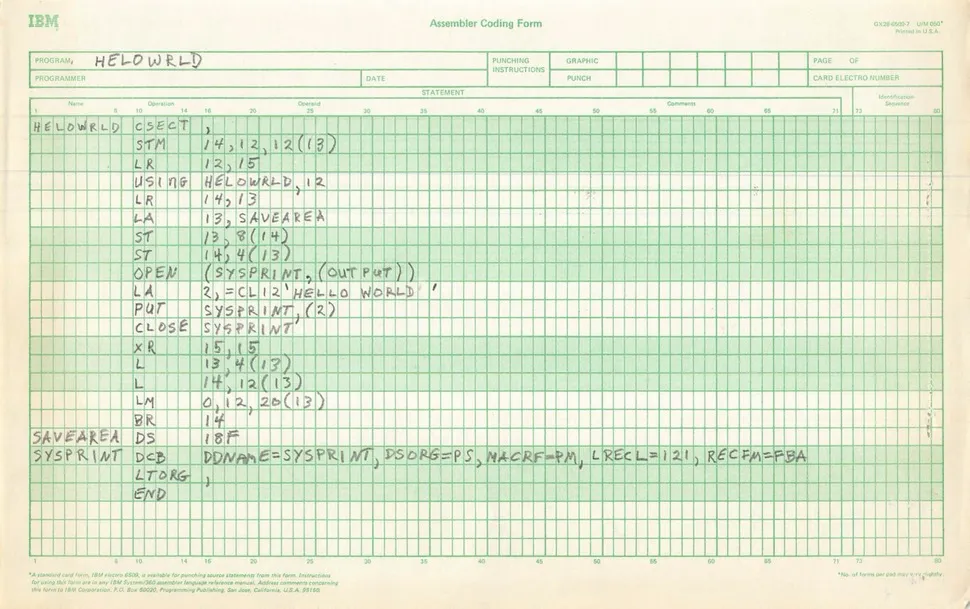
\includegraphics[width=13cm]{src/build/codingsheet.png}}%
    \caption{An example of a coding sheet to give you an idea of what programming was like in 1981.}
\end{figure}

If you fill out enough of these sheets with 6502 assembly you have a program that can be typed out and assembled. 
\begin{definition}[dave says\index{dave says}]
\setlength{\intextsep}{0pt}%
\setlength{\columnsep}{3pt}%
\begin{wrapfigure}{l}{0.12\textwidth}
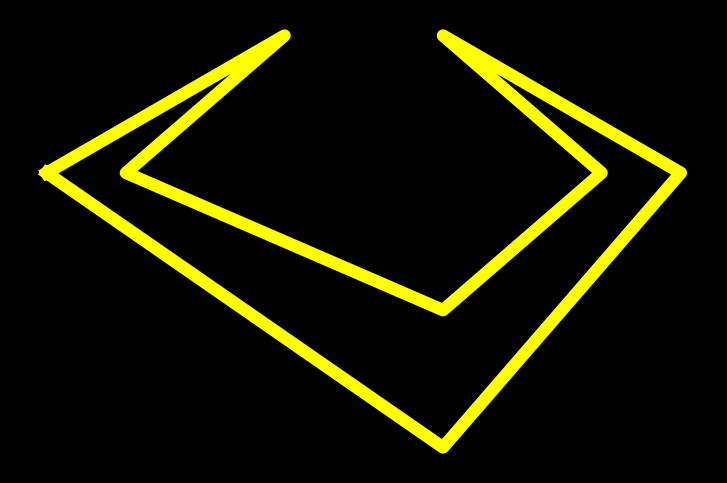
\includegraphics[width=\linewidth]{src/callout/claw_t.png} 
\end{wrapfigure}
\small
\textcolor{white}{
I’d write the code on programming sheets and turn it in to the typists
who’d type them in to a DEC computer, then give us a tape with the resulting
compiled/linked program.
}
\end{definition}

Once the typists had entered your program into the PDP-11 in building 1360 the would see a listing
of the files such as this on a VT-100 terminal.
\begin{figure}[H]
      \centering
      \frame{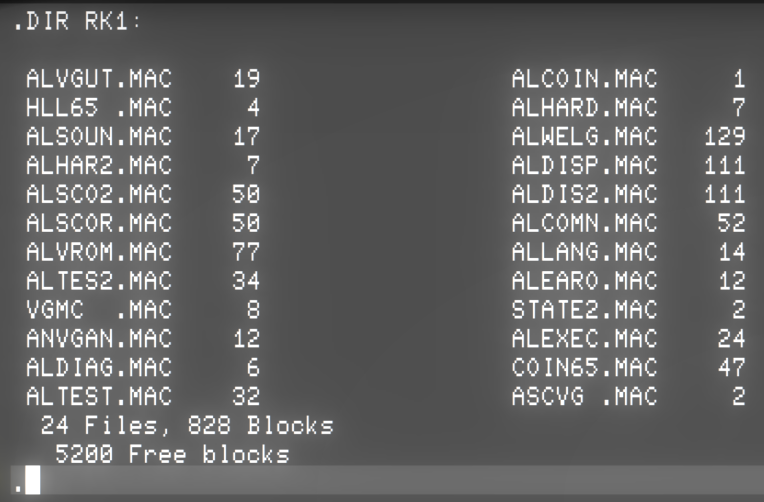
\includegraphics[width=12cm]{src/build/dir.png}}%
    \caption{Listing the Tempest source files.}
\end{figure}

Their next step was to assemble each of the files using the \icode{MAC65} command on each:
\begin{figure}[H]
      \centering
      \frame{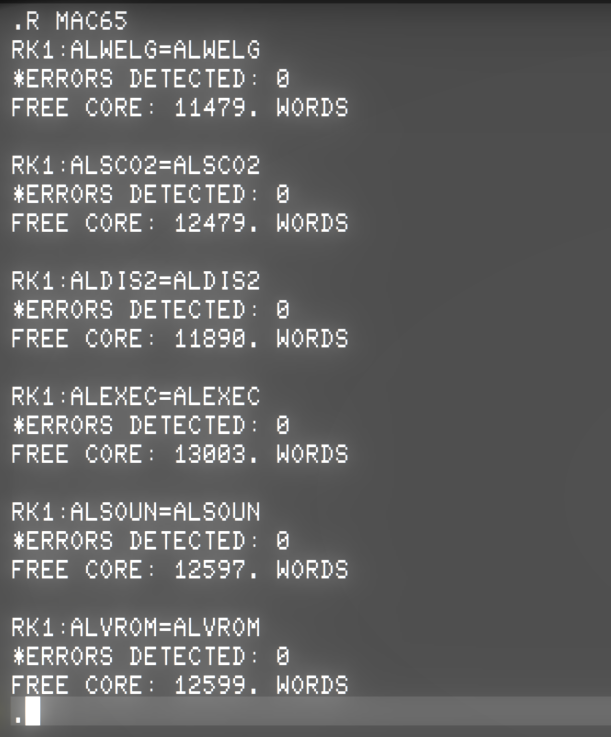
\includegraphics[height=7cm]{src/build/assemble1.png}}%
      \frame{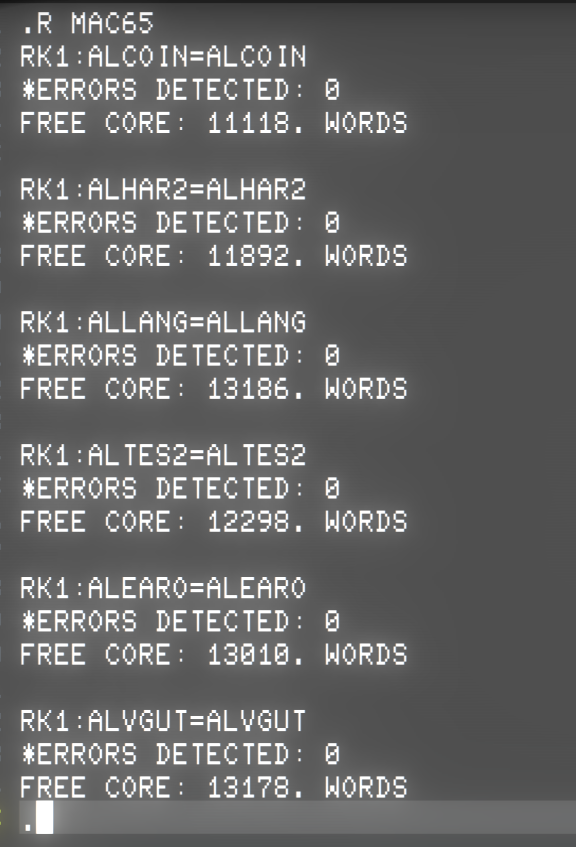
\includegraphics[height=7cm]{src/build/assemble2.png}}%
    \caption{Assembling the Tempest source files.}
\end{figure}

Once that was done they could run the \icode{RMAC} command to link the assembled files into a
single object file \icode{ALEXEC.LDA}.
\begin{figure}[H]
      \centering
      \frame{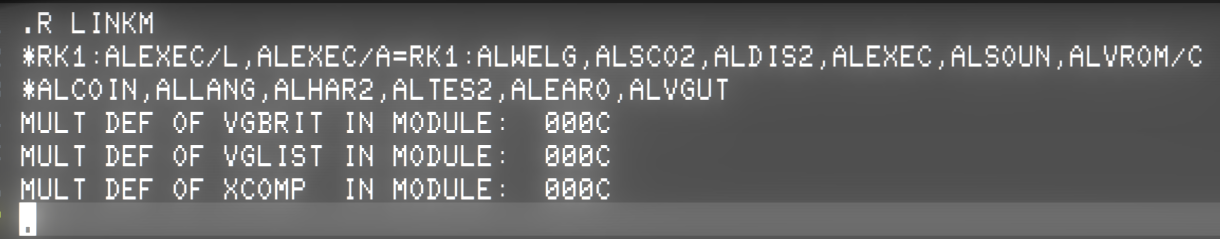
\includegraphics[width=12cm]{src/build/link.png}}%
    \caption{Linking the Tempest object files.}
\end{figure}

\begin{definition}[dave says\index{dave says}]
\setlength{\intextsep}{0pt}%
\setlength{\columnsep}{3pt}%
\begin{wrapfigure}{l}{0.12\textwidth}
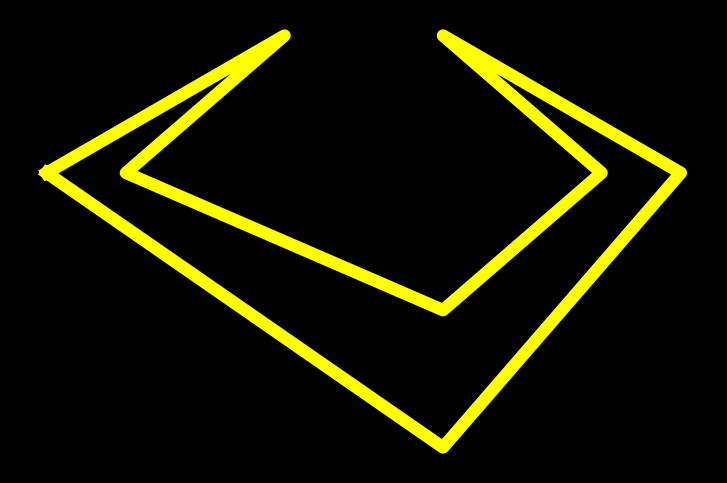
\includegraphics[width=\linewidth]{src/callout/claw_t.png} 
\end{wrapfigure}
\small
\textcolor{white}{
We’d then take that to a blue box [which used the
FORTH programming language] for debugging. We’d mark changes to the code on a
listing, give it back to the typists who’d edit our files and give us a new
tape. Repeat ad infinitum.
}
\end{definition}

Once you have completed the ad-infinitum phase of this process you may have a game that is ready
for production and distribution. For this you must talk to your project manager, Morgan, and together
decide how to split the \icode{ALEXEC.LDA} file into a number of different files. Each of these will
be written to a specific ROM chip as detailed by the parts manifest you devise together and distribute to
the guys in building 1320:
\begin{figure}[H]
      \centering
      \frame{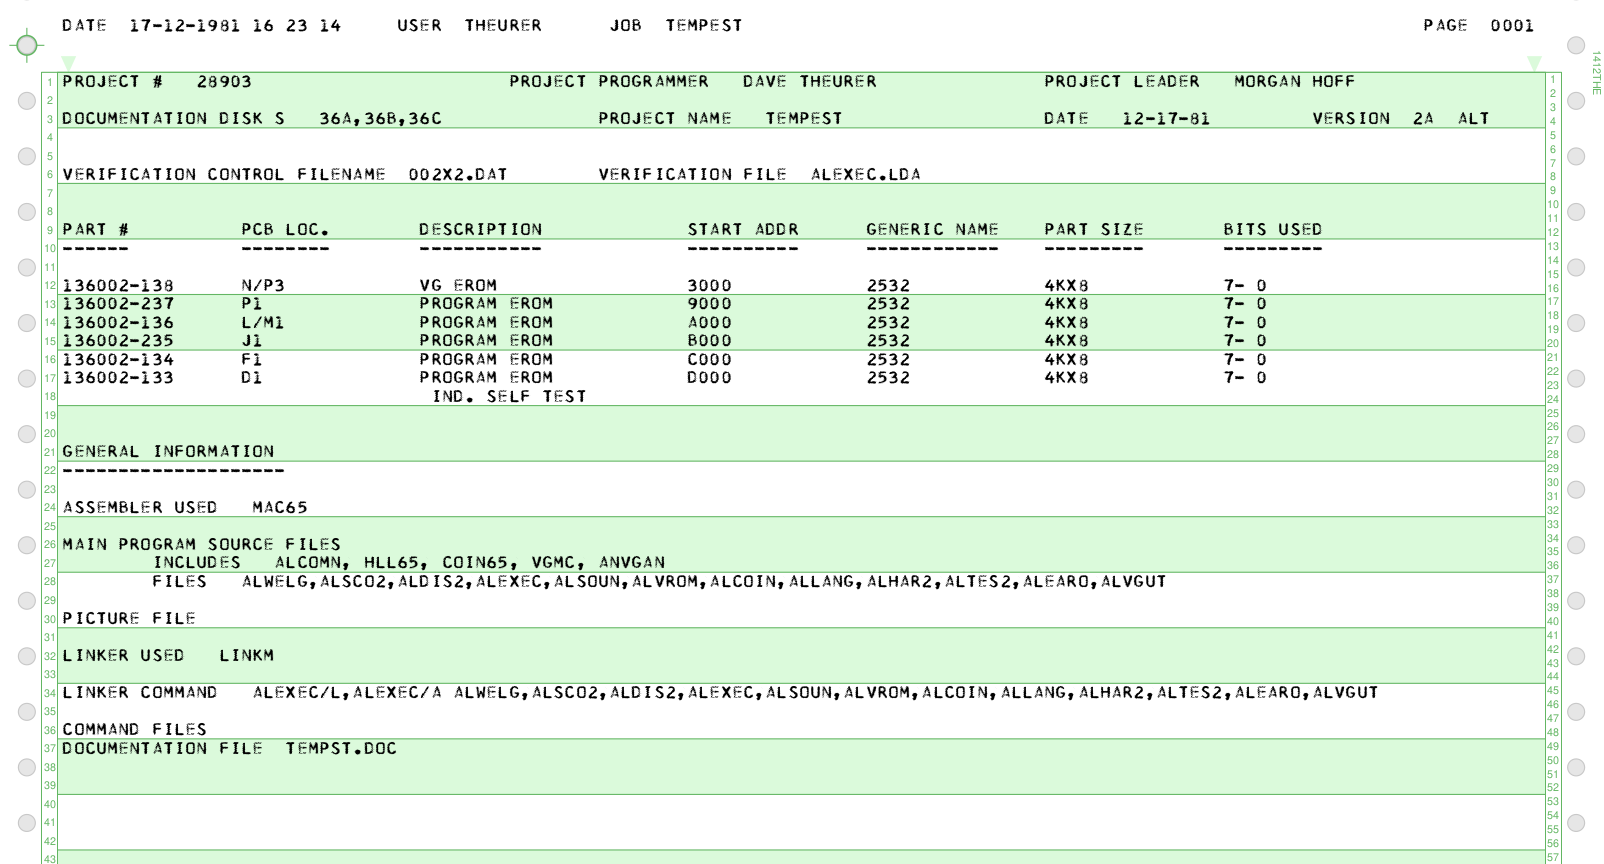
\includegraphics[width=13cm]{src/build/tempst.doc.png}}%
    \caption{The actual build manifest for Tempest, recreated in the style of the time.}
\end{figure}

You might expect that splitting \icode{ALEXEC.LDA} is as simple as carving up its raw contents into these
component files. You would be wrong. \icode{ALEXEC.LDA} actually consists of a long sequence of triplets, 
each giving you the ROM address a set of bytes are to be written to, the number of bytes, followed by the
bytes themselves. This table shows the first ten or so triplets to give you an idea of what we mean. 
\icode{ALEXEC.LDA} contains 2000 such triplets in total!

\begin{figure}[H]
  {
    \setlength{\tabcolsep}{3.0pt}
    \setlength\cmidrulewidth{\heavyrulewidth} % Make cmidrule = 
    \begin{adjustbox}{width=12cm,center}

      \begin{tabular}{lll}
        \toprule
        Address & Length & Data\\
        \midrule
        \icode{9000} & 38 & \icode{02BB5A3050EE3DA84D20C592203492202B902031A8A9FA855BA9008D0601855FA90085016020} \\
        \icode{9026} & 38 & \icode{1B9220C592208F92206F92204692209F9220AD92206EC1A9FF8D24018D4801A9008D230160A9} \\
        \icode{904C} & 19 & \icode{108D0202A9008529852BAD2101852A1000C62B} \\
        \icode{905C} & 1 & \icode{02} \\
        \icode{905F} & 38 & \icode{A201A52A0A662A6629CA10F6A529186D22018D2201A52A65688568A52B65698569A55F186918} \\
        \icode{9085} & 17 & \icode{855FA55B6900855BC9FC9000A9018D1501} \\
        \icode{9090} & 1 & \icode{05} \\
        \icode{9096} & 11 & \icode{A55F38E55DA55BF000E9FF} \\
        \icode{909E} & 1 & \icode{02} \\
        \icode{90A1} & 18 & \icode{D000A55D855FA9FF855BA90424053000A908} \\
        \icode{90B0} & 1 & \icode{02} \\
        \icode{90B3} & 9 & \icode{8500A63DA9009D0201} \\
        \icode{90A2} & 1 & \icode{19} \\
        \icode{90BC} & 36 & \icode{A9FF8D14014C4997AD2601A21CCADDFE9190FAA004AD6A012904F000AD1D07C9309000C8} \\
        \icode{90DE} & 1 & \icode{01} \\
        \icode{90E0} & 5 & \icode{C9509000C8} \\
        \icode{90E3} & 1 & \icode{01} \\
        \icode{90E5} & 5 & \icode{C9709000C8} \\
        \icode{90E8} & 1 & \icode{01} \\
        \icode{90D7} & 1 & \icode{12} \\
        \icode{90EA} & 10 & \icode{A5092943C940D000A01B} \\
        \icode{90F1} & 1 & \icode{02} \\
        \icode{90F4} & 8 & \icode{8429E429B000A629} \\
        \icode{90F9} & 1 & \icode{02} \\
        \icode{90FC} & 12 & \icode{8E2701A5051000A9008D2601} \\
        \icode{9102} & 1 & \icode{05} \\
        \icode{9108} & 9 & \icode{A63F863DF00020B292} \\
        \icode{910D} & 1 & \icode{03} \\
        \icode{9111} & 38 & \icode{A904857CA9FF855BA9008D00028551857B8D0506A6051000A9148D0506A9FF8D1101A9168500} \\
        \icode{9137} & 13 & \icode{A9088501A900859F2096C1A910} \\
        \icode{9128} & 1 & \icode{1B} \\
        \bottomrule
      \end{tabular}
    \end{adjustbox}
  }\caption*{The triplets in \icode{ALEXEC.LDA} for ROM address \icode{9000} written to ROM Part 136002-237.}
\end{figure}
\vspace{-0.5cm}
Notice how apparently wasteful this file format is: some of the triplets contain only byte! You can also notice
that the triplets can appear out of order. For example the bytes for address \icode{90A2} are specified after the 
bytes for \icode{90A1}. So perhaps for some binaries this encoding scheme may be more efficient than just raw bytes,
but not in the case of \icode{ALEXEC.LDA} which uses 25,408 bytes to encode a total of 24,576 bytes that actually
get written to the ROM parts on the circuit board.

Which leads nicely to our final diagram. If you look closely in the circuit board diagram on the following page you
will find the final destination for these files in the printed circuit board shipped in the arcade cabinet. They
are the parts indicated by stars at the top of the board.
\begin{figure}[H]
      \centering
      \frame{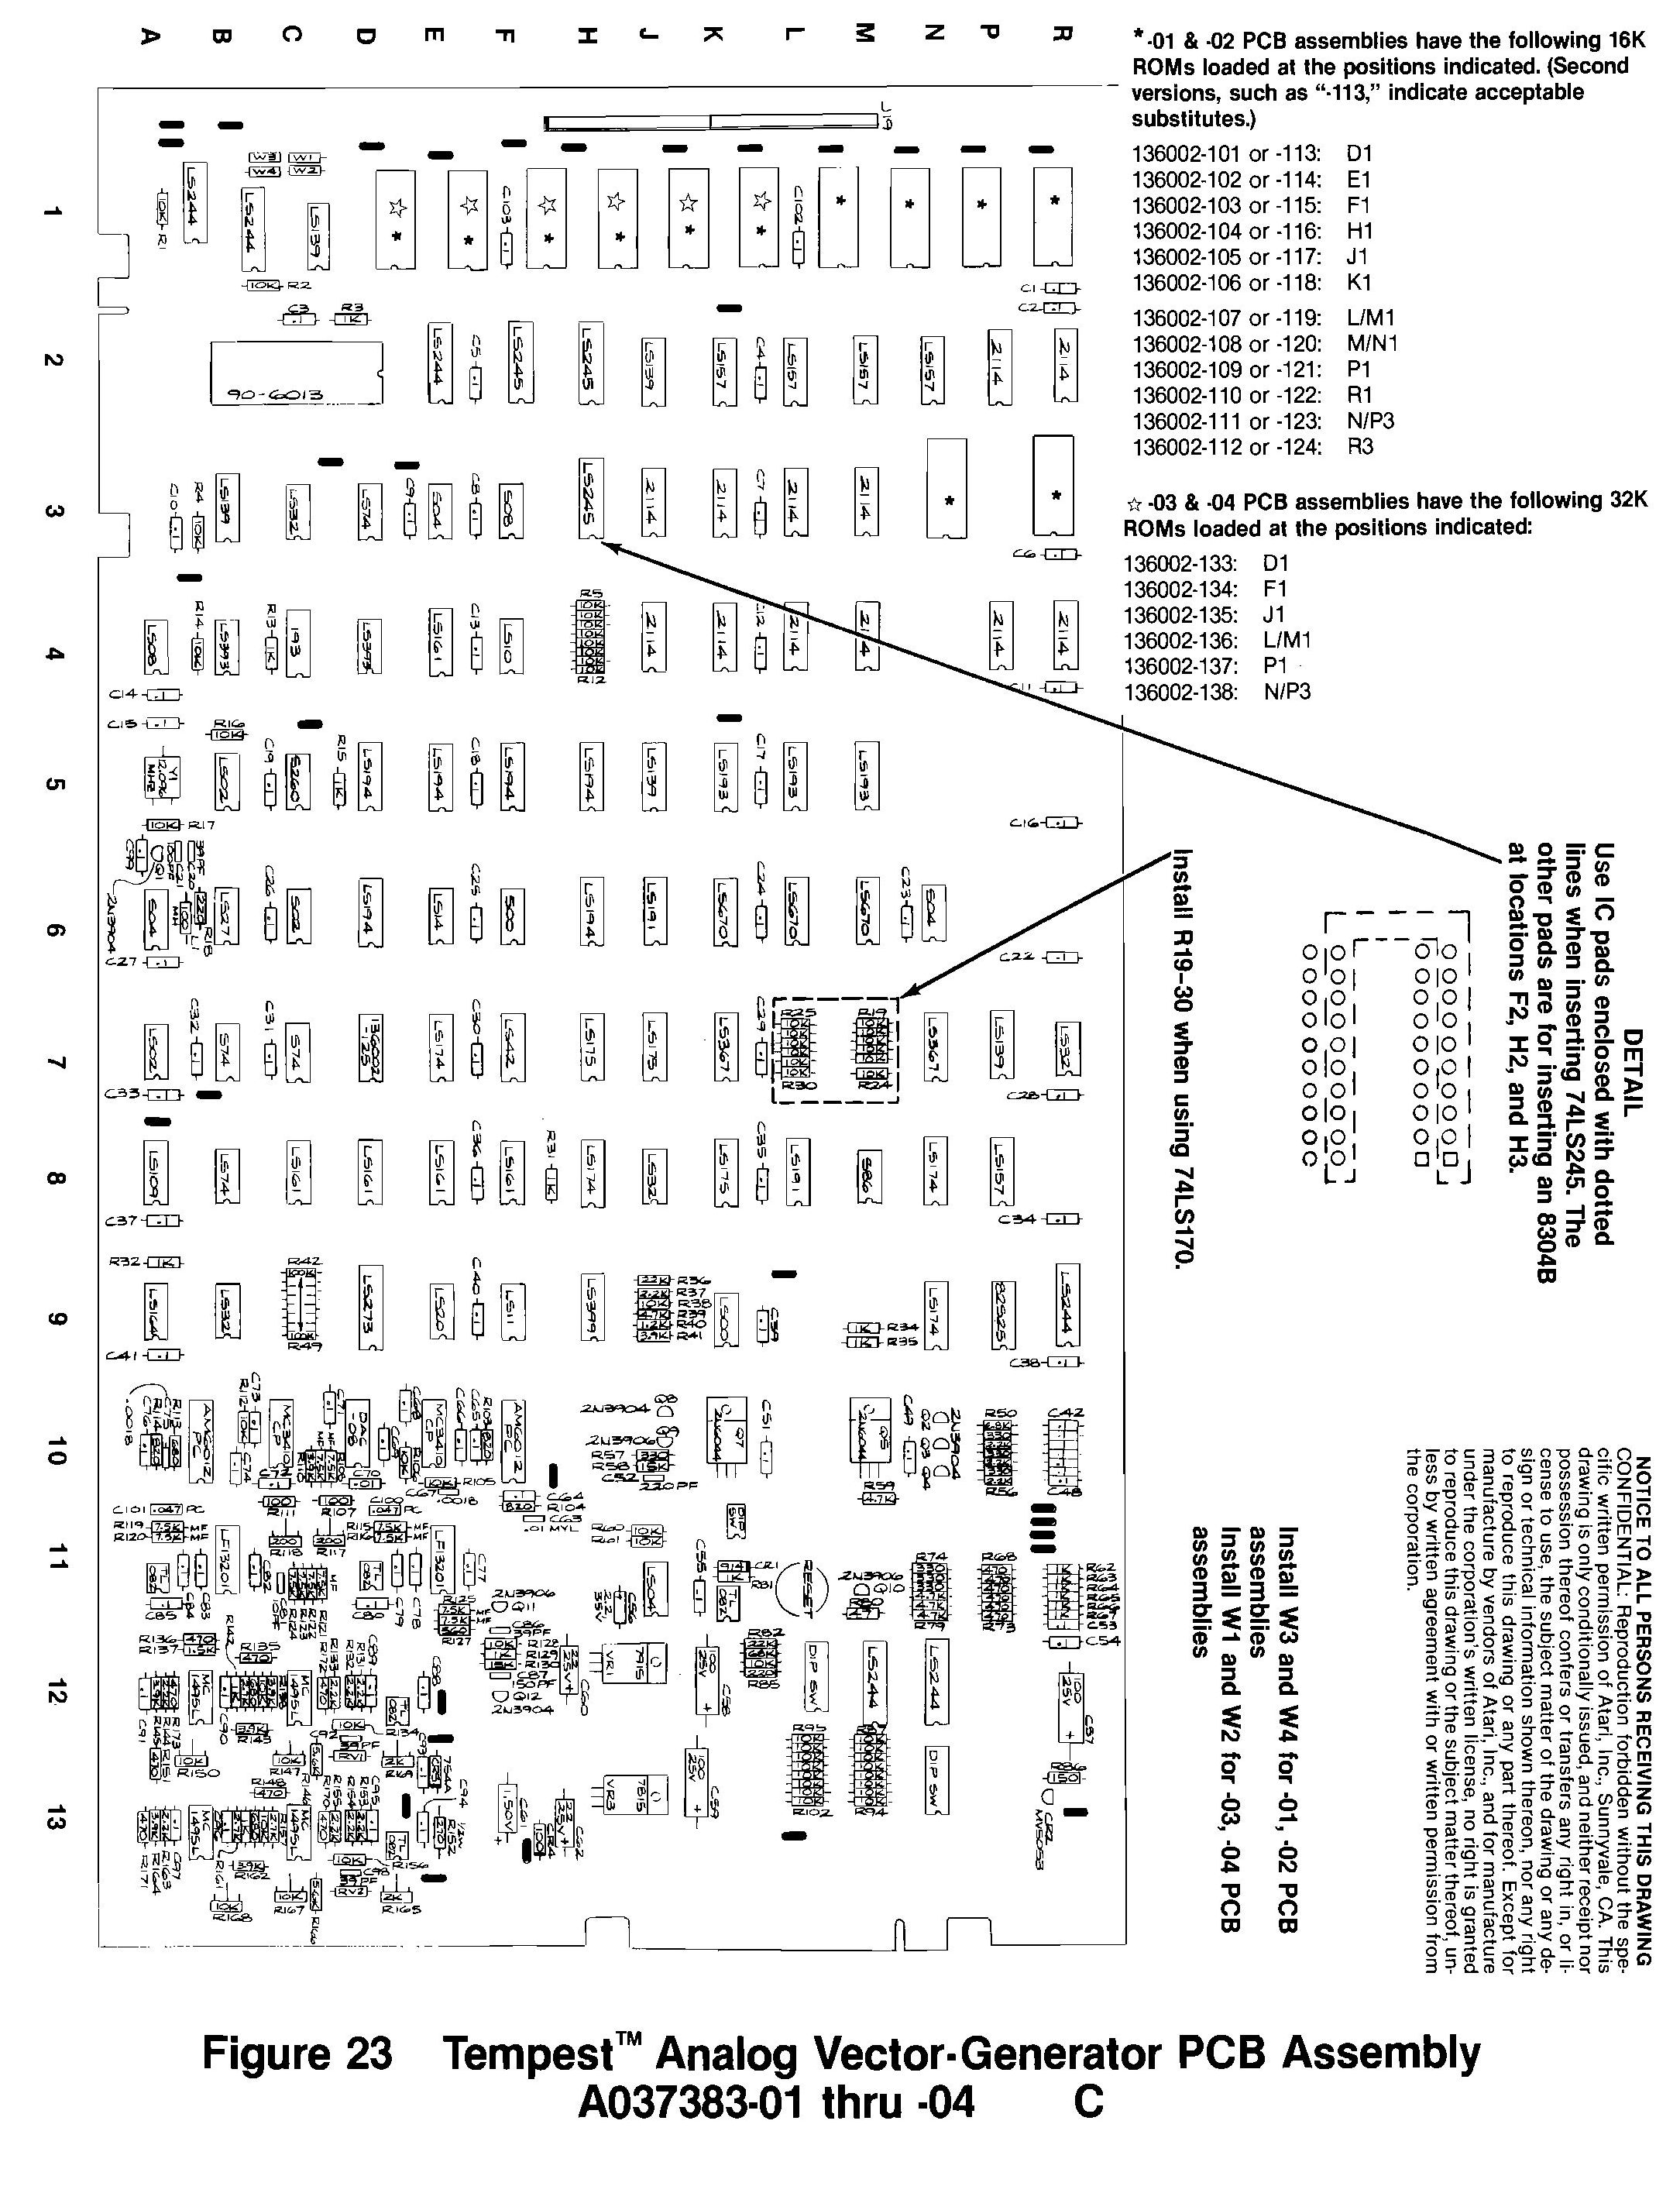
\includegraphics[width=13cm]{src/build/pcb.jpg}}%
    \caption{The circuit board diagram containing the ROM chips that our ROM files are written to..}
\end{figure}

\begin{figure}[H]
      \centering
      \frame{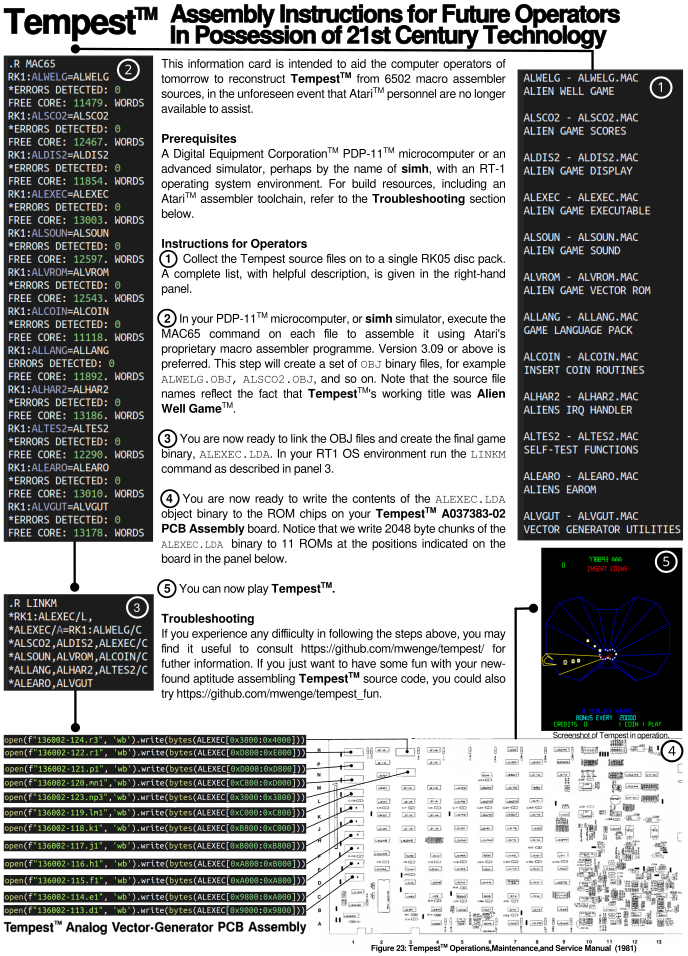
\includegraphics[width=13cm]{src/build/PagedOut-TempestBuild.png}}%
    \caption{Information Card describing the build process on modern systems.}
\end{figure}
